%++++++++++++++++++++++++++++++++++++++++
% Don't modify this section unless you know what you're doing!
\documentclass[letterpaper, 12pt]{article}
\usepackage{tocstyle}
\usepackage{listings}
\usepackage[T1]{fontenc}
\usepackage[margin=1in]{geometry} % 1 inch margins
\setlength{\parskip}{.8em}
\usepackage{tabularx} % extra features for tabular environment
\usepackage{amsmath}  % improve math presentation
\usepackage{graphicx} % takes care of graphic including machinery
% \usepackage[margin=1in,letterpaper]{geometry} % decreases margins
\usepackage{cite} % takes care of citations
\usepackage[final]{hyperref} % adds hyper links inside the generated pdf file
\usepackage[utf8]{inputenc}
\usepackage{cprotect}
\hypersetup{
	colorlinks=false,      % false: boxed links; true: colored links
	linkcolor=blue,        % color of internal links
	citecolor=blue,        % color of links to bibliography
	filecolor=magenta,     % color of file links
	urlcolor=blue
}

\usetocstyle{standard}
\settocstylefeature[-1]{pagenumberbox}{\csname @gobble\endcsname} % no page numbers for part

\usepackage{menukeys}

\usepackage{color}
\usepackage{caption}

\usepackage{xcolor}
\usepackage{textcomp}

\definecolor{dkgreen}{rgb}{0,0.6,0}
\definecolor{gray}{rgb}{0.5,0.5,0.5}
\definecolor{mauve}{rgb}{0.58,0,0.82}

\lstset{
    frame=none,
    language=C,
    aboveskip=10mm,
    belowskip=10mm,
    showstringspaces=false,
    columns=flexible,
    keepspaces=true,
    basicstyle=\small\ttfamily,
    numbers=none,
    numberstyle=\tiny\color{gray},
    keywordstyle=\color{blue},
    commentstyle=\color{dkgreen},
    stringstyle=\color{mauve},
    breaklines=true,
    breakatwhitespace=true,
    tabsize=4,
    upquote=true,
}

\newcounter{nalg}[section] % defines algorithm counter for chapter-level
\renewcommand{\thenalg}{\arabic{nalg}} %defines appearance of the algorithm counter
\DeclareCaptionLabelFormat{algocaption}{Pseudocode \thenalg} % defines a new caption label as Algorithm x.y

\lstnewenvironment{pseudocode}[1][] %defines the algorithm listing environment
{
    \refstepcounter{nalg} %increments algorithm number
    \captionsetup{labelformat=algocaption,labelsep=colon} %defines the caption setup for: it ises label format as the declared caption label above and makes label and caption text to be separated by a ':'
    \lstset{ %this is the stype
        mathescape=true,
        frame=tB,
        numbers=left,
        numberstyle=\tiny,
        basicstyle=\scriptsize,
        keywordstyle=\color{black}\bfseries\em,
        keywords={,input, output, return, datatype, function, in, if, else, foreach, for, while, begin, end, print, in, of, not, call, is,} %add the keywords you want, or load a language as Rubens explains in his comment above.
        numbers=left,
        escapeinside={<@}{@>},
        xleftmargin=.04\textwidth,
        stringstyle=\color{black},
        #1 % this is to add specific settings to an usage of this environment (for instance, the caption and referable label)
    }
}
{}

\renewcommand*\contentsname{Table of Contents}

%++++++++++++++++++++++++++++++++++++++++


\begin{document}

\title{\vspace{30mm}EE474: LAB ASSIGNMENT 1}
\author{Conor Sayres, and José Sánchez-Gallego}
\date{\today}

\maketitle

\thispagestyle{empty}

\clearpage

\tableofcontents
\thispagestyle{empty}

\clearpage


\section{ABSTRACT}

This document describes the work and results obtained for the first laboratory assignment for EE474. We were introduced to some simple examples of code in C, which we modified, debugged, and repurposed. In the process we learned the use of the GNU compiler and debugger, and wrote our first, simple C applications.


\section{INTRODUCTION}

The purpose of this assignment is to understand basic concepts of the C language, as well as to design our first applications based on design requirements. This is also a good opportunity to become familiar with the BeagleBone environment for development, the GNU compiler, and the debugger.

Section \ref{sec:design} defines the design specifications for the project. The software implementation of each one of the subprojects is discussed in Section \ref{sec:implementation}. Testing is discussed in Section \ref{sec:design_testing}. Our main results are presented in \ref{sec:results}. Errors are discussed in Section \ref{sec:errors}. We provide our summary and conclusions in Sections \ref{sec:summary} and \ref{sec:conclusions}, respectively.


\section{DESIGN SPECIFICATIONS}
\label{sec:design}

The work for Lab Assignment 1 is specified in lab1Summer17.pdf under the three following headings:

\begin{enumerate}
    \item  Building, Editing, and Running a Program
    \item  Working With the Debugger
    \item Building Your Own Applications
\end{enumerate}

We will generally present this work in the order in which it is outlined in the assignment.

\subsection{Stepwise Modifications of Project 1a}
\label{sec:stepwise_mod_spec}

Building, Editing, and Running a Program outlines a stepwise modification of the provided C program:  project1a-2017.c.  This program will print the numbers 9 through 0 separated by a space in turn on a single output line in a console.  A delay function is implemented in the code such that the numbers appear at a rate that a human can read.  After  the countdown from 9 to 0 is complete, the program removes each number in the order it was printed from the terminal display, again with a delay for human readability.

The specified modification steps to this code are outlined below (codes for each of these steps are discussed and provided later in this document):

\begin{enumerate}
    \item Annotate, compile, and run the program.
    \item Parameterize the delay() function.
    \item Replace  the two for loops with  functions.
    \item Pass a delay parameter by reference, rather than value.
    \item Combine the two looping functions into a single function.
    \item Breakout the single looping function into a separate file.
\end{enumerate}

\subsection{Debugging Projects 1b and 1c}
Codes project1b-2017.c and project1c-2017.c both contain errors.  Use the debugger to identify any problems, and provide code that corrects these problems.

\subsection{Building Your Own Applications}
This section asks the student to create three applications by reworking what it has been learned in previous sections:

\begin{itemize}
    \item \textbf{Application 1:} write a program that writes \verb+A B C D+ to the standard output and flashes the letters at a one-second interval.
    \item \textbf{Application 2:} modify application 1 to write and erase each one of the letters at a one-second rate.
    \item \textbf{Application 3:} modify application 1 to flash the letters \verb+A+ and \verb+C+ at a one-second rate and \verb+B+ and \verb+D+ at a two-second rate.
\end{itemize}


\section{SOFTWARE IMPLEMENTATION}
\label{sec:implementation}

\subsection{Stepwise Modifications of Project 1a}
Here we provide a C program and discussion for each requirement enumerated in
Section \ref{sec:stepwise_mod_spec}.  Each subsequent section contains code that has been modified from the previous section to satisfy the requirements outlined above.
\subsubsection{Annotate, compile, and run the program.}
Code: project1a-2017-annotated.c.  This is a version of the provided project1a-2017.c code that is more clearly annotated, and somewhat cleaned up.  It was compiled and run and shown to behave as expected on the beaglebone.
\subsubsection{Parameterize the delay() function.}
Code: project1a-2017-param-delay.c.  This program parameterizes the delay values separately for printing and erasing the numbers on console.  Default delay values for both are set to 1000.  The user may override these values at the command line by specifying 1 or 2 command line arguments of type unsigned int.  They will override the print and erase delay time respectively.  Example usage setting print delay to 2000 and erase delay to 3000:

\begin{lstlisting}[language=bash]
  $ gcc project1a-2017-param-delay.c
  $ ./a.out 2000 3000
\end{lstlisting}

\subsubsection{Replace  the two for loops with  functions.}
Code: project1a-2017-function-loops.c.  This code moves each for loop in the main function into two separate functions, which are then called from main.  Code snippets:
\begin{lstlisting}[language=C]
int main(int argc, char *argv[])
{
   ...
   while(TRUE)
   {
      f1Data(delayValuePrint); // write numbers
      f2Clear(delayValueClear); // clear numbers
   }
   ...
}
void f1Data(unsigned long delay1)
{
   char myData[3];
   for (int i = 9; i >=0; i--)
   {
      myData[0] = i + '0';        //  convert the int i to ascii
      myData[1] = '\0';           //  terminate the string
      printf("%s ", myData);      //  add the current value of i to the stdout buffer
      fflush(stdout);             //  flush the buffer so the value is displayed to the user
      delay(delay1);                //  delay so we can read the display
   }

   //  print a carridge return, bringing us back to the beginning of the output line
   printf("%c", 0x0d);
   fflush(stdout);
}
void f2Clear(unsigned long delay2)
{
   for (int i = 0; i < 10; i++)
   {
      printf("%s ", " \0");  // add the space to the stdout buffer
      fflush(stdout);         // show the user
      delay(delay2);            // delay so we can read the display
   }
   //  print a carridge return, bringing us back to the beginning of the output line
   printf("%c", 0x0d);           //  print a carridge return
   fflush(stdout);
}
\end{lstlisting}

\subsubsection{Pass a delay parameter by reference, rather than value.}
Code: project1a-2017-pointer-reference.c.  The modification here is to simply pass the delay value by reference rather than by value.   This is shown in the following  snippets:
\begin{lstlisting}[language=C]
int main(int argc, char *argv[])
{
   ...
   while(TRUE)
      {
         f1Data(&delayValuePrint); // write numbers
         f2Clear(&delayValueClear); // clear numbers
      }
    ...
 }
void f1Data(unsigned long *delay1)
{
  ...
}
void f2Clear(unsigned long *delay2)
{
   ...
}
\end{lstlisting}

\subsubsection{Combine the two looping functions into a single function.}
Code: project1a-2017-single-function.c.  This code combines the two looping functions into a single function: \textbf{dataLoop}.  This function accepts two parameters: a delay value, and a boolean flag.  The delay value corresponds to the delay between subsequent number prints or erases.  The flag indicates whether this loop function will print numbers or erase existing numbers.  The assignment specifications called for a function with arguments for a character to display and the desired delay value, this in implemented in the function \textbf{delayedWrite}.   We found this combination of functions (\textbf{dataLoop} calling \textbf{delayedWrite}) as a nice way to oranize this program.  Code snippets indicating the design are shown below:
\begin{lstlisting}[language=C]
int main(int argc, char *argv[])
{
   ...
   while(TRUE)
      {
         dataLoop(&delayValuePrint, 1); // write numbers
         dataLoop(&delayValueClear, 0); // clear numbers
      }
    ...
 }
void dataLoop(unsigned long *delayValue, int showNumber)
{
   int i = 0; // initialize loop vairable
   // initialize it as an empty space
   char myData[3] = " \0";
   // loop from 9 to 0
   for (i = 9; i >=0; i--)
   {
      if (1 == showNumber)
      {
         // populate myData with the integer if flag is set
         myData[0] = i + '0';        //  convert the int i to ascii
         myData[1] = '\0';           //  terminate the string
      }
      delayedWrite(delayValue, myData); // write to the user
      }

      //  print a carridge return, bringing us back to the beginning of the output line
      printf("%c", 0x0d);
      fflush(stdout);
}

void delayedWrite(unsigned long *delayValue, char *data)
{
   printf("%s ", data);  // print the data to the user
   fflush(stdout);
   delay(*delayValue);   // delay so we can read the display
}
\end{lstlisting}


\subsubsection{Breakout the single looping function into a separate file.}
Code: project1a-2017-external.c, delayedWrite.c.  The  final modification of this code was to breakout  the \textbf{delayedWrite} function into a  separate file.   It is specified in delayedWrite.c, and  called in project1a-2017-external.c.  A line was added to  the main program file:
\begin{lstlisting}[language=C]
extern void delayedWrite(unsigned long *delayValue, char *data);
\end{lstlisting}
and the  code was compiled and run like so:
\begin{lstlisting}[language=bash]
  $ gcc delayedWrite.c project1a-2017-external.c
  $ ./a.out 2000 3000
\end{lstlisting}
We use this final incarnation of project1a-2017.c as an example in Section \ref{sec:results}.

\subsection{Debugging Project 1b and 1c.}
Please see Section \ref{sec:design} for discussion on the debugging excercises.  These excercises were intended for practice with the gdb debugger and recognizing and correcting a couple common programming mistakes in the C language.

\subsection{Build your own applications.}

This sections describes how we implemented the software design for applications 1 to 3. All the applications require a delay function that blocks the execution flow for an integer number of seconds. This is difficult to accomplish using the \verb+delay()+ function introduced in the previous examples, which is sensitive to CPU performance and system load. Instead, we replaced the \verb+delay()+ function with the following code (the full code is available in file \verb+delay.c+).

\begin{lstlisting}
void delay (unsigned int a_delay) {
    // Waits a_delay seconds before returning.

    unsigned int return_time = time(0) + a_delay;  // Return time
    while (time(0) < return_time);                 // Loops until return time
}
\end{lstlisting}

This function determines the time at which the function should return (defined as the current time plus a number of \verb+a_delay+ seconds) and loops until that moment.

The following subsections discuss the software implementation of each one of the applications.

\subsubsection{Application 1.}

Application 1 is a relatively simple rewrite of the previous examples. The following pseudocode shows the implementation, which can be found in full in file \verb+applications/app1.c+. Note that, for simplicity, this pseudocode (and the others in this section) do not show the commands to flush the standard output.

\begin{pseudocode}[caption={Application 1 pseudocode.}, label={app1}]
 input: nothing
 output: nothing
 begin
   while True
     print "A<@\textvisiblespace@>B<@\textvisiblespace@>C<@\textvisiblespace@>D"
     call delay()
     print <@\return@>
     print "<@\textvisiblespace@><@\textvisiblespace@><@\textvisiblespace@><@\textvisiblespace@>"
     call delay()
     print <@\return@>
   end
 end
\end{pseudocode}

\noindent where \return{} represents a carriage return and \textvisiblespace{} is a space.

\subsubsection{Application 2.}

Application 2 involves writing the letters \verb+A B C D+ in order on a one-second interval, and then removed them at the same rate. This is similar to project1a and can be accomplished using similar code. The following pseudocode sketches how that would be done.

\begin{pseudocode}[caption={Application 2 pseudocode (not implemented).}, label={app2_notused}]
 input: nothing
 output: nothing
 begin
    while True
        foreach ii of (A B C D)
            print ii
            print <@\textvisiblespace@>
            call delay()
        end
        print <@\return@>
        for ii = 1 to 4
            print ii
            print <@\textvisiblespace@>
            call delay()
        end
        print <@\return@>
    end
 end
\end{pseudocode}

This code can be simplified in the following manner.

\begin{pseudocode}[caption={Application 2 pseudocode (implemented).}, label={app2}]
 input: nothing
 output: nothing
 begin
    characters $\gets$ "<@\return@>ABCD<@\return@><@\textvisiblespace@><@\textvisiblespace@><@\textvisiblespace@><@\textvisiblespace@>"
    while True
        foreach char of characters
            print char
            print <@\textvisiblespace@>
            call delay()
        end
    end
 end
\end{pseudocode}

The full implementation for Pseudocode \ref{app2} can be found in file \verb+applications/app2.c+.

\subsubsection{Application 3.}

In this application we print the same letters as in the previous applications but switch them on or off depending on the iteration. Letters \verb+A+ and \verb+C+ are switched every second and \verb+B+ and \verb+D+ every two seconds.

To accomplish that we make each iteration one second long and print or not each specific letter depending on the evenness of the iteration.

\begin{pseudocode}[caption={Application 2 pseudocode (implemented).}, label={app2}]
 input: nothing
 output: nothing
 begin
    write_AC $\gets$ True
    write_BD $\gets$ True
    counter $\gets$ 0
    characters $\gets$ "ABCD"
    while True
        foreach char of characters
            if (char is A or C) and (write_AC is True)
                print char
            end
            if (char is B or D) and (write_BD is True)
                print char
            end
            print <@\textvisiblespace@>
            call delay()
        end
        print <@\return@>
        write_AC $\gets$ (not write_AC)
        if counter is not even
            write_BD $\gets$ (not write_BD)
        end
    end
 end
\end{pseudocode}


\section{DESIGN TESTING}
\label{sec:design_testing}

All code was compiled and successfully run on the BeagleBone. In all cases we compiled out code using the flags \verb+-Wall -Wextra -O2+. These flags provide extra warnings which are useful for debugging. In particular, the \verb+-O2+ flag enables some compiler optimisation that, as a result, issues a warning if an array is trying to write to a memory address that does not belong to the user. This was useful for debugging project1b.

For project1a and applications 1 to 3 we did not need to use the debugger; we run the codes in the BeagleBone and checked that their behaviour was the expected one.

For project1b we used the gdb debugger, setting break points inside the for loops, and printing the value of \verb+i+. We also used the function \verb+seizeof+ to determine the size of the \verb+myArray+ array. In this way we determined that the array had a length of five elements while the for loop was setting six values (the ASCII representation of letters A to F). In the BeagleBone, the result of compiling and running the original code is the expected one (letters A to F are printed). When compiling the code with flags \verb+-Wall -Wextra -O2+, we get

\begin{verbatim}
project1b-2017.c:16:19: warning: iteration 5 invokes undefined behavior
[-Waggressive-loop-optimizations]
     myArray[i]= 65+i;
     ~~~~~~~~~~^~~~~~
\end{verbatim}

\noindent which pinpoints the problem. The solution to this problem is easy, we modify the declaration of \verb+myArray+ to be six elements long.

It is worth mentioning that the behaviour of the original code (before fixing the bug) depends on the version of the compiler. For instance, in the BeagleBone, which uses gcc 4.6.3, when we run the code we obtain the expected six letters, A to F. The same code, compiled and run with gcc 7.1.0 on a Mac computer produces the letters A to E, with an empty character as the last line.

\begin{figure}[!ht]
  \centering
  \captionsetup{width=0.8\textwidth}
  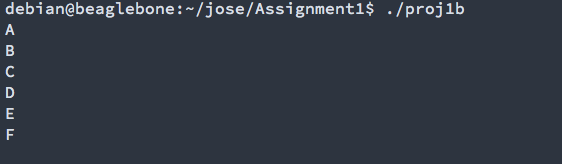
\includegraphics[width=0.6\textwidth]{images/proj1b_beagle.png}
  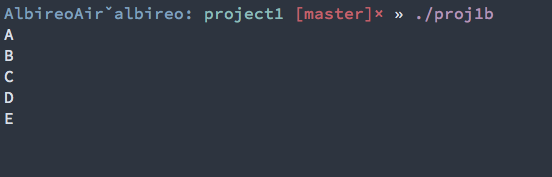
\includegraphics[width=0.6\textwidth]{images/proj1b_mac.png}
  \cprotect\caption{Original code for \verb+project1b.c+ compiled and run on the BeagleBone (top) and MacOS 10.11 with GCC 7.1.0 (botom).}
  \label{fig:proj1b}
\end{figure}

\verb+project1c.c+ presents a different kind of problem. In that example, the pointer \verb+myPtr+ is used to store a value obtained from the user in the variable \verb+myValue+. The original code does not work because the memory address to which \verb+myPtr+ points is overwritten in the function \verb+getData()+ to point to \verb+tempValue+. Commenting the line \verb+valuePtr = &tempValue;+ is enought to make the code work. Again, the debugger is useful in this case. By setting a break point after \verb+*valuePtr = getchar();+ we were able to print the values of \verb+*valuePtr+, \verb+myValue+, and \verb+tempValue+ to understand why the code was not working.


\section{PRESENTATION AND RESULTS}
\label{sec:results}
\subsection{Stepwise Modifications of Project 1a}
Presented below is example of compilation, usage, and output for the last iteration of modifications for project 1a.   The  executable is compiled from two separate files, the delay times are passed as command line arguments to the program.  Figure \ref{fig:proj1a} displays screen shots during different times during the execution of the program.

\begin{figure}[!ht]
  \centering
  \captionsetup{width=0.8\textwidth}
  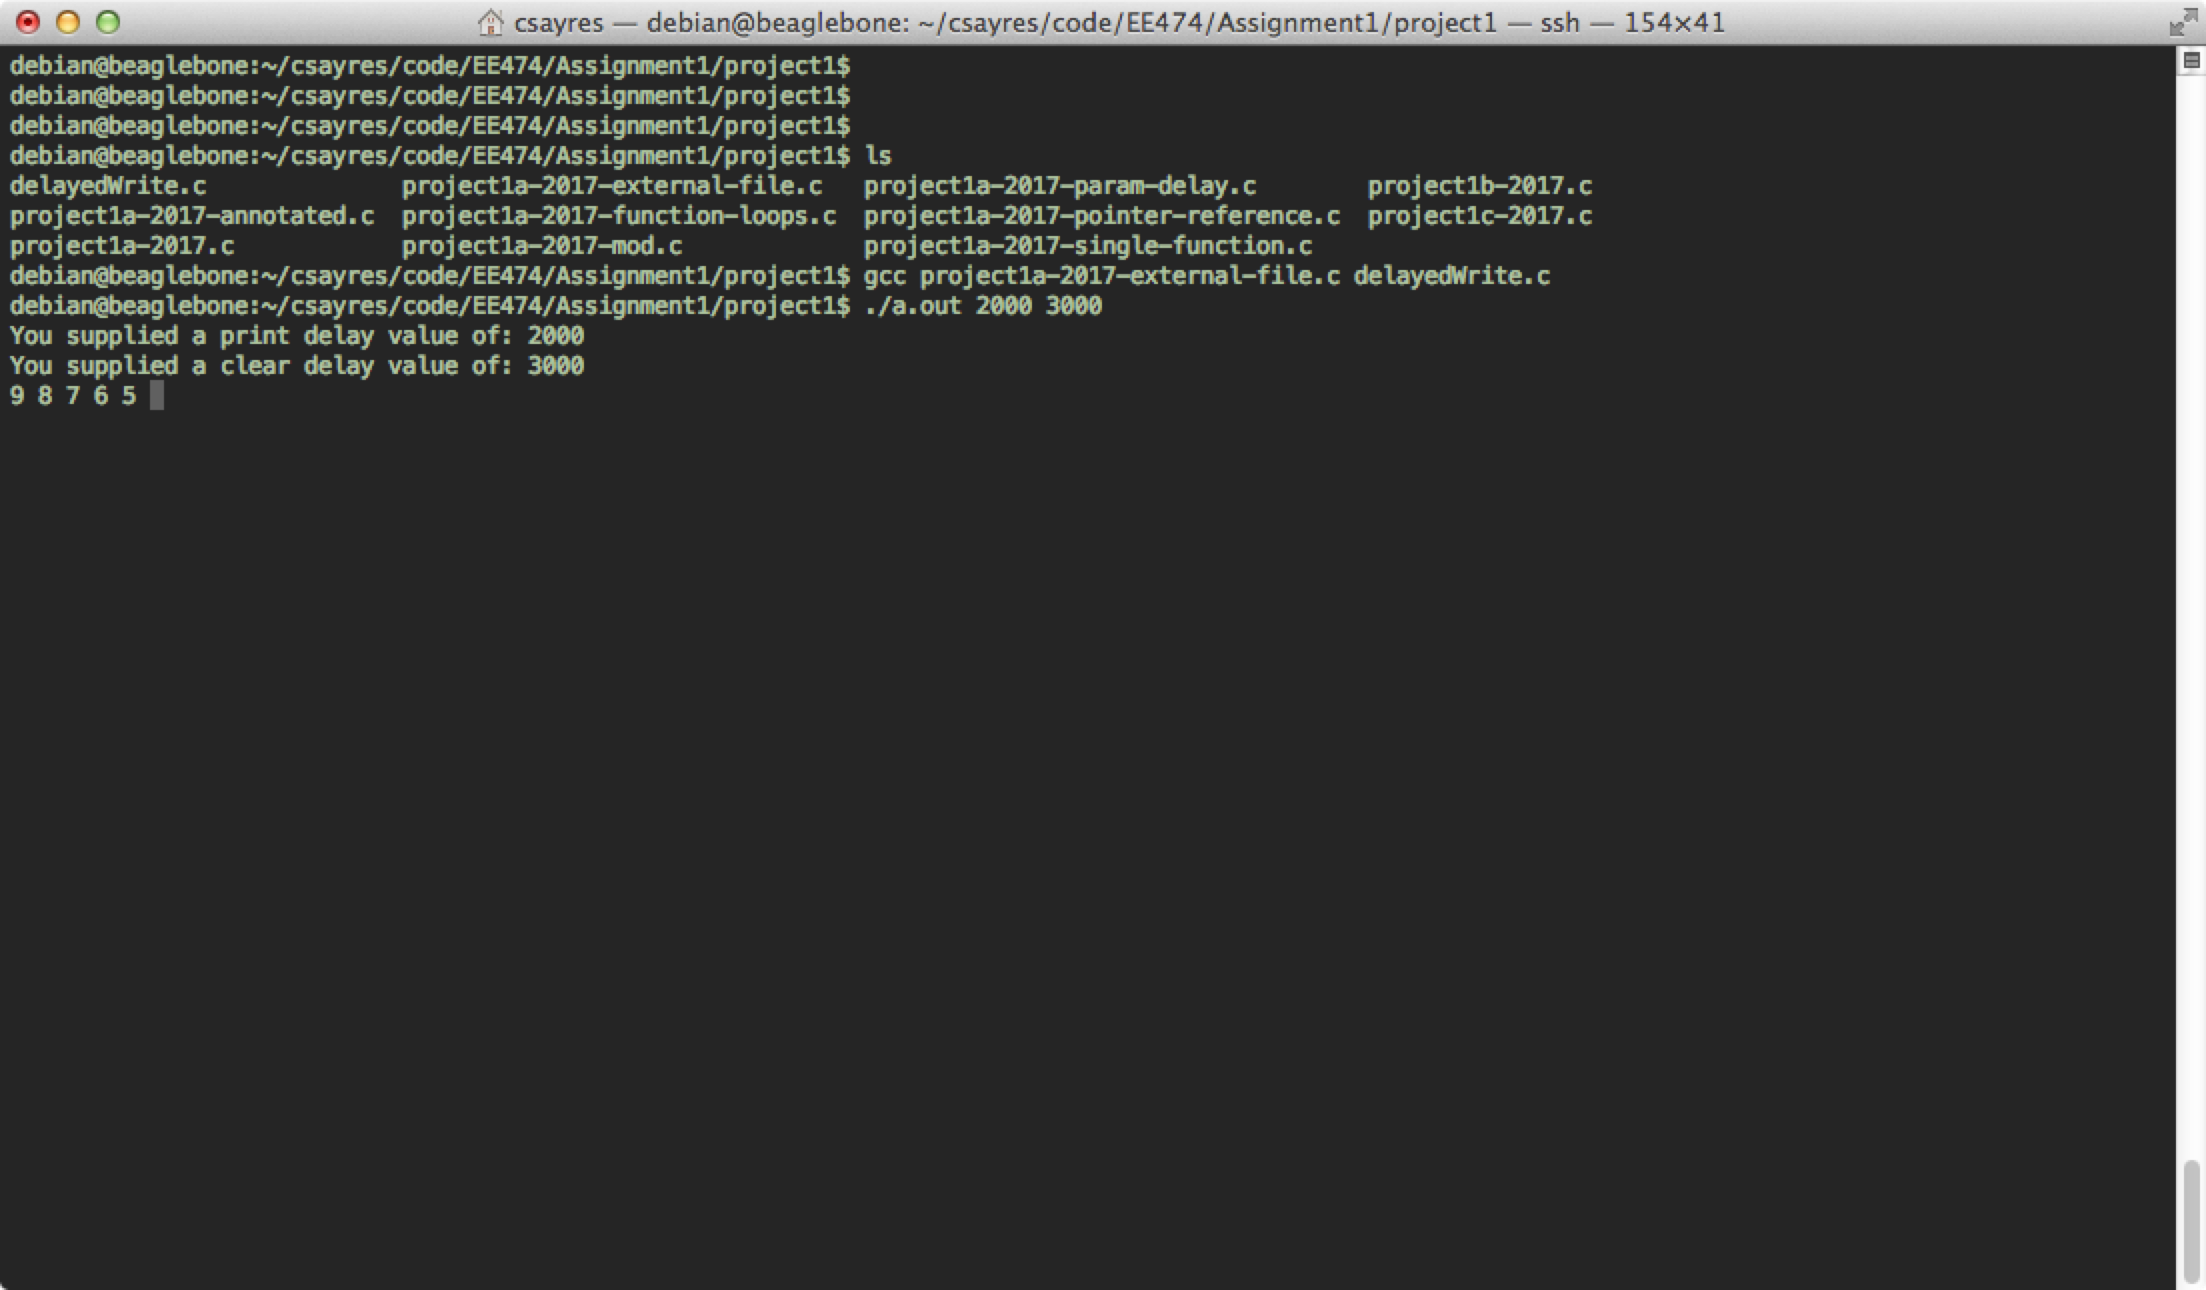
\includegraphics[width=0.6\textwidth]{images/ss1.png}
  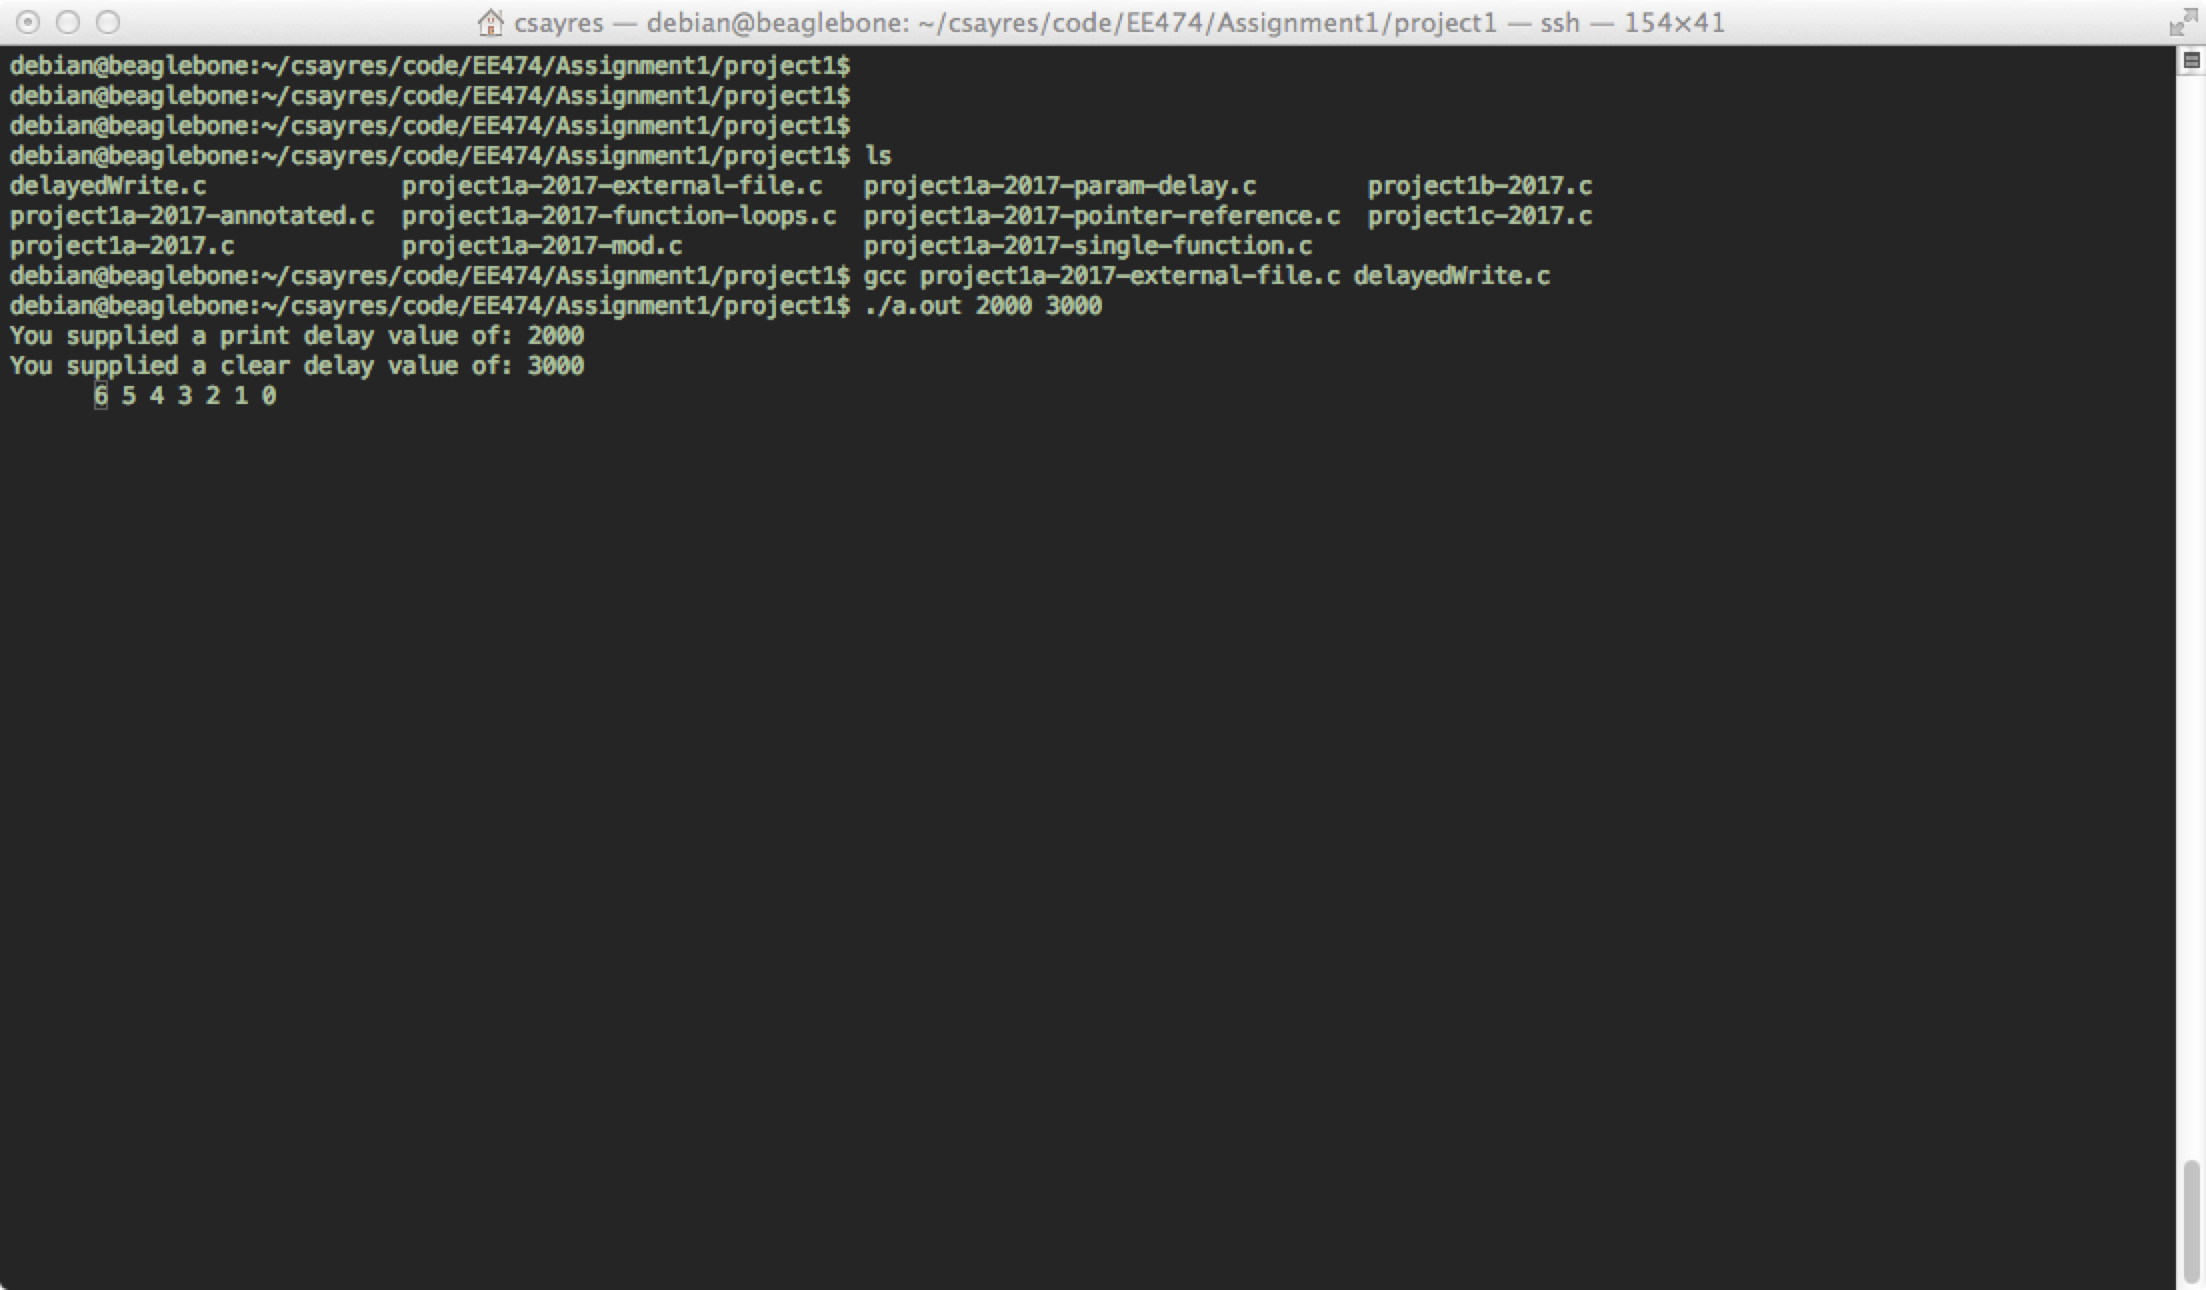
\includegraphics[width=0.6\textwidth]{images/ss2.png}
  \cprotect\caption{Different steps during the execution of \verb+project1a+.}
 \label{fig:proj1a}
\end{figure}

\subsection{Debugging Projects 1b and 1c.}
Output of project 1b has been discussed in Section \ref{sec:design_testing} and example output is displayed in Figure \ref{fig:proj1b}.  Note that the code would  run without obvious issue on the BeagleBone despite the presence of a common C programming array indexing mistake.  We have included the corrected code with this report.  Output from the corrected  code for project 1c code is shown in  Figure \ref{fig:proj1c}.

\begin{figure}[!ht]
  \centering
  \captionsetup{width=0.8\textwidth}
  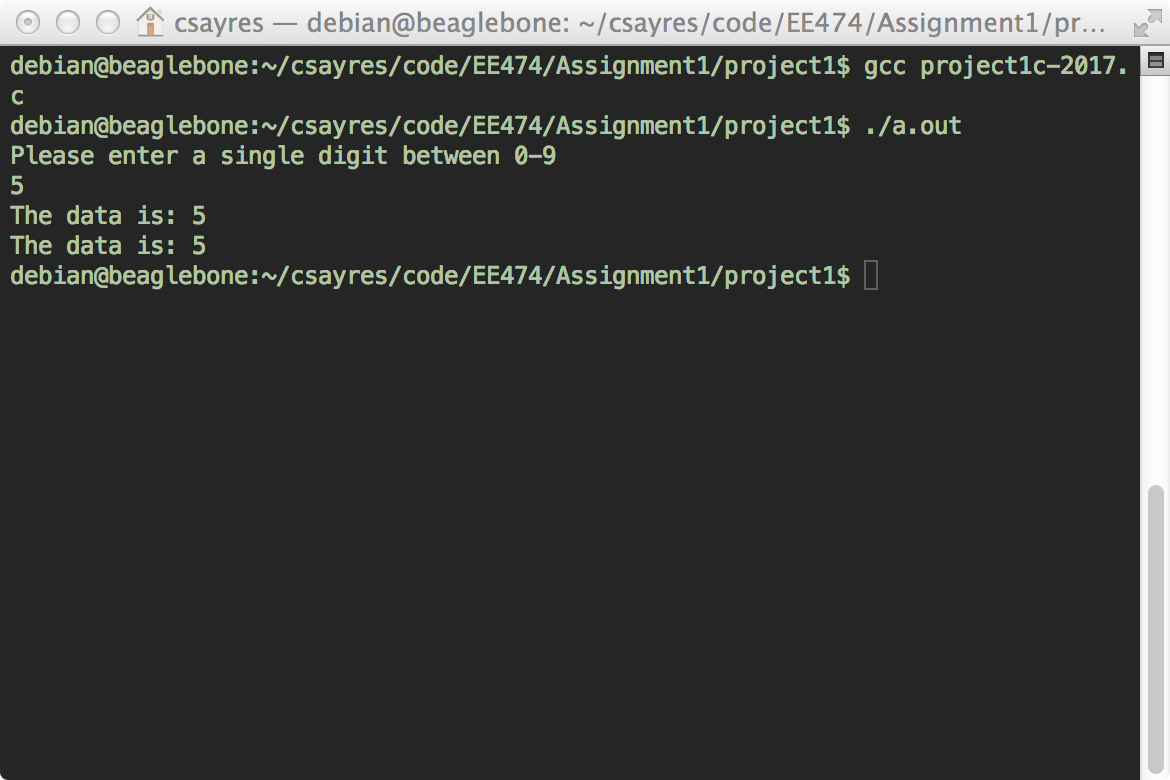
\includegraphics[width=0.6\textwidth]{images/proj1c.png}
  \cprotect\caption{Example of correctly executing \verb+project1c+ program.}
 \label{fig:proj1c}
\end{figure}

\subsection{Build your own applications.}

Here we describe the results obtained for applications 1 to 3.  In these particular cases there is not much to discuss beyond making sure the code compiles without error (or significant warnings) and the results shown on the terminal are what we expect.

We compile the code for application 1 by running

\begin{verbatim}
gcc -Wall -Wextra -O2 app1.c delay.c -o app1
\end{verbatim}

\noindent The following figure shows some screenshots of the code running.

\begin{figure}[!ht]
  \centering
  \captionsetup{width=0.8\textwidth}
  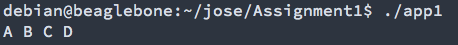
\includegraphics[width=0.6\textwidth]{images/app1_1.png}
  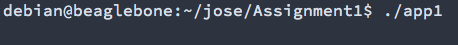
\includegraphics[width=0.6\textwidth]{images/app1_2.png}
  \cprotect\caption{Result of running \verb+app1+ compiled from \verb+app1.c+. The top and bottom screenshots shows the letters flashing at a one second interval.}
\end{figure}

We compile and execute the other applications similarly. Figures \ref{fig:app2} and \ref{fig:app3} shows the result of running applications 2 and 3.

\begin{figure}[!ht]
  \centering
  \captionsetup{width=0.8\textwidth}
  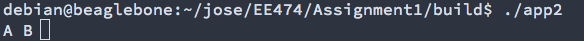
\includegraphics[width=0.6\textwidth]{images/app2_1.png}
  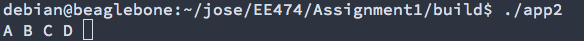
\includegraphics[width=0.6\textwidth]{images/app2_2.png}
  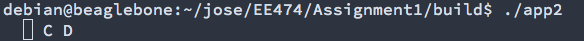
\includegraphics[width=0.6\textwidth]{images/app2_3.png}
  \cprotect\caption{Different steps during the execution of \verb+app2+ compiled from \verb+app2.c+.}
\end{figure}

\begin{figure}[!ht]
  \centering
  \captionsetup{width=0.8\textwidth}
  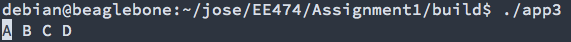
\includegraphics[width=0.6\textwidth]{images/app3_1.png}
  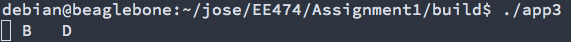
\includegraphics[width=0.6\textwidth]{images/app3_2.png}
  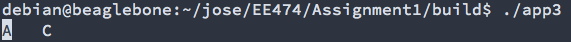
\includegraphics[width=0.6\textwidth]{images/app3_3.png}
  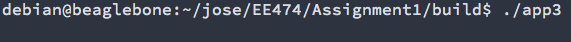
\includegraphics[width=0.6\textwidth]{images/app3_4.png}
  \cprotect\caption{Different steps during the execution of \verb+app3+ compiled from \verb+app3.c+.}
\end{figure}

\section{ANALYSIS OF ERRORS}
\label{sec:errors}

We did not encounter any significant error apart from the typical typos and syntax problems. We debugged those issues, in particular project1b and project1d, as explained in Section \ref{sec:design_testing}, with the help of the compiler output and the debugger.


\section{SUMMARY}
\label{sec:summary}

All our applications and codes work as expected based on the design requirements described in Section \ref{sec:design}. The codes in \verb+project1b.c+ and \verb+project1c.c+ have been debugged and fixed to work consistently with all versions of the GNU C compiler and architectures.


\section{CONCLUSION}
\label{sec:conclusions}

While working on this assignment we have become familiar with a number of basic concepts in the C language. We have been able to compile, execute, debug, and repurpose existing code to implement several applications based on design requirements. We have become familiar with the GCC compiler and debugger, and the BeagleBone environment. While most of the concepts and applications described in this report are relatively simple, this assignment represents a good stepping stone for more complex projects and applications.

\clearpage

\hypertarget{appendixstart}{\appendix} % Make a anchor here
\addtocontents{toc}{
    \protect\contentsline{part}{
        \protect\hyperlink{appendixstart}{Appendices}
    }{}{}
}

\section{CONTRIBUTION}

Both team members wrote code separately for every piece of assigned work.  Final codes presented here were selected, modified, and/or combined from each team member's individual codes.  Both team members wrote and revised equal content  in this document.

For this project we did not need to include any specific appendix, since all the snippets of code are short and included in their relevant sections, and the screenshots are shown in Section \ref{sec:results}. The full code is provided as a separate deliverable.

\end{document}
